% Created 2020-05-27 Wed 12:51
% Intended LaTeX compiler: pdflatex
\documentclass[presentation]{beamer}
\usepackage[utf8]{inputenc}
\usepackage[T1]{fontenc}
\usepackage{graphicx}
\usepackage{grffile}
\usepackage{longtable}
\usepackage{wrapfig}
\usepackage{rotating}
\usepackage[normalem]{ulem}
\usepackage{amsmath}
\usepackage{textcomp}
\usepackage{amssymb}
\usepackage{capt-of}
\usepackage{hyperref}
\usetheme{UoB}
\author{Mark Blyth}
\date{\textit{[2020-05-27 Wed]}}
\title{The codimension of pseudo-plateau bursting}
\hypersetup{
 pdfauthor={Mark Blyth},
 pdftitle={The codimension of pseudo-plateau bursting},
 pdfkeywords={},
 pdfsubject={},
 pdfcreator={Emacs 26.3 (Org mode 9.1.9)}, 
 pdflang={English}}
\begin{document}

\maketitle

\section{Background}
\label{sec:org008afe7}
\subsection{SUMMARY}
\label{sec:org5c584bc}
\begin{frame}[label={sec:org503af10}]{Paper goals}
\begin{itemize}
\item Determine the codimension-classification of pseudo-plateau bursting
\item Propose a normal form for bursting
\end{itemize}
\vfill
\end{frame}

\begin{frame}[label={sec:org2a0ea87}]{Plan de jour}
\begin{itemize}
\item \alert{30 second intro to neurons}
\begin{itemize}
\item \alert{What do neurons do?}
\item \alert{What are bursting neurons?}
\item \alert{How and why do we categorise them?}
\end{itemize}
\item Section 2: Towards a normal form for bursting
\item Section 3: Transitions between bursting classes
\item Section 4:Codimension-classification of pseudo-plateau bursting
\item Section 5: Conclusion
\end{itemize}
\end{frame}

\subsection{What are bursters?}
\label{sec:org0e94b0b}
\begin{frame}[label={sec:org9d76c7d}]{Neurons spike}
\begin{center}
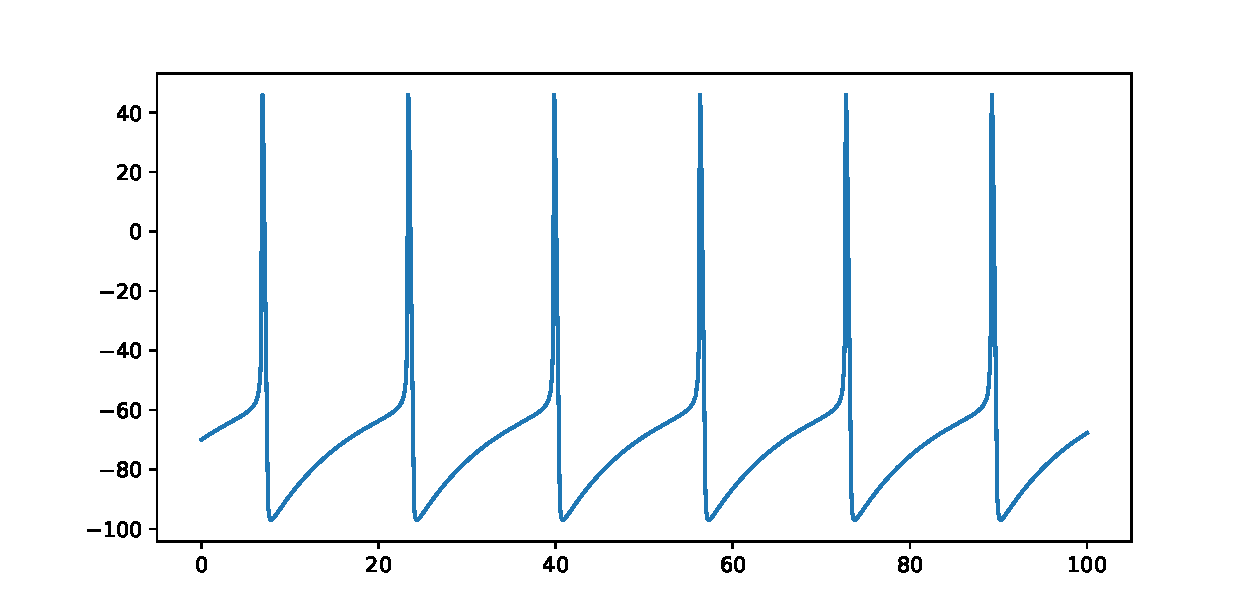
\includegraphics[width=.9\textwidth]{./HHraw.pdf}
\end{center}

Neurons encode information in action potentials
\end{frame}


\begin{frame}[label={sec:org32906a5}]{Ionic currents}
\begin{center}
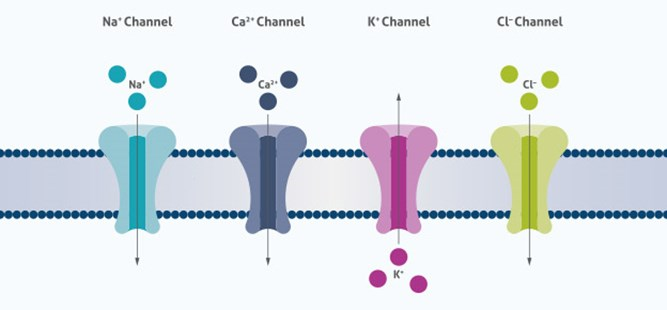
\includegraphics[width=.9\textwidth]{./voltage-gated.jpg}
\end{center}

Action potentials happen from ions flowing into and out of the cell
\end{frame}


\begin{frame}[label={sec:org45bbdfd}]{Hodgkin-Huxley}
\begin{eqnarray}
\frac{dV}{dt} &=& \left[I_{inj} - \bar{g}_{Na}m^3h(V-V_{Na}) -\bar{g}_Kn^4(V-V_K) - g_L (V-V_L)\right]/C\nonumber\\
\frac{dn}{dt} &=& \alpha_n(V) (1-n) - \beta_n(V)n\nonumber\\
\frac{dm}{dt} &=& \alpha_m(V) (1-m) - \beta_m(V)m\nonumber\\
\frac{dh}{dt} &=& \alpha_h(V) (1-h) - \beta_h(V)h\nonumber  
\end{eqnarray}

\vfill

We can understand the causes of spike generation with differential equations
\end{frame}




\begin{frame}[label={sec:orgd4faa9a}]{Nonlinear dynamics}
\begin{center}
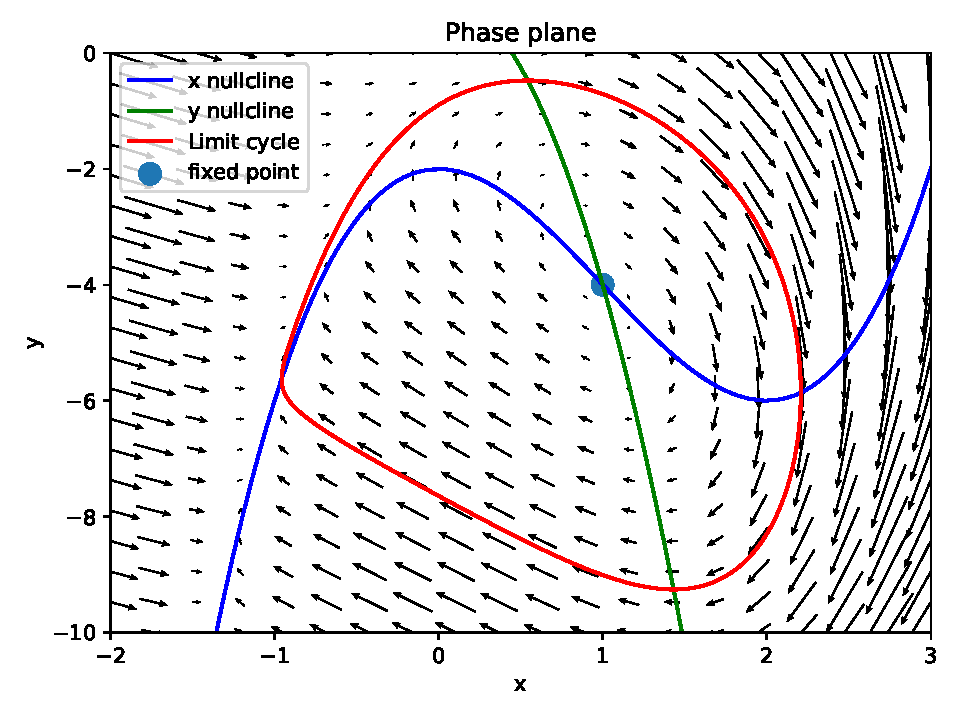
\includegraphics[trim={0cm 0.5cm 0cm 0cm}, clip,height=.75\textheight]{./phaseplane.pdf}
\end{center}

Neuron dynamics rely on limit cycles and equilibria
\end{frame}


\begin{frame}[label={sec:orge7a70e4}]{Bifurcations}
\begin{center}
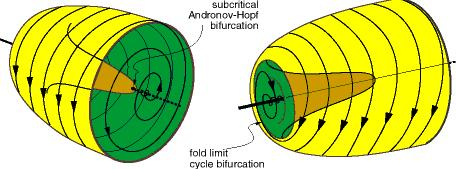
\includegraphics[width=.9\linewidth]{./Ellburst.jpg}
\end{center}

Equilibria and limit cycles an appear through bifurcations
\end{frame}


\begin{frame}[label={sec:org85dab1a}]{KEY POINT: bursting}
\begin{center}
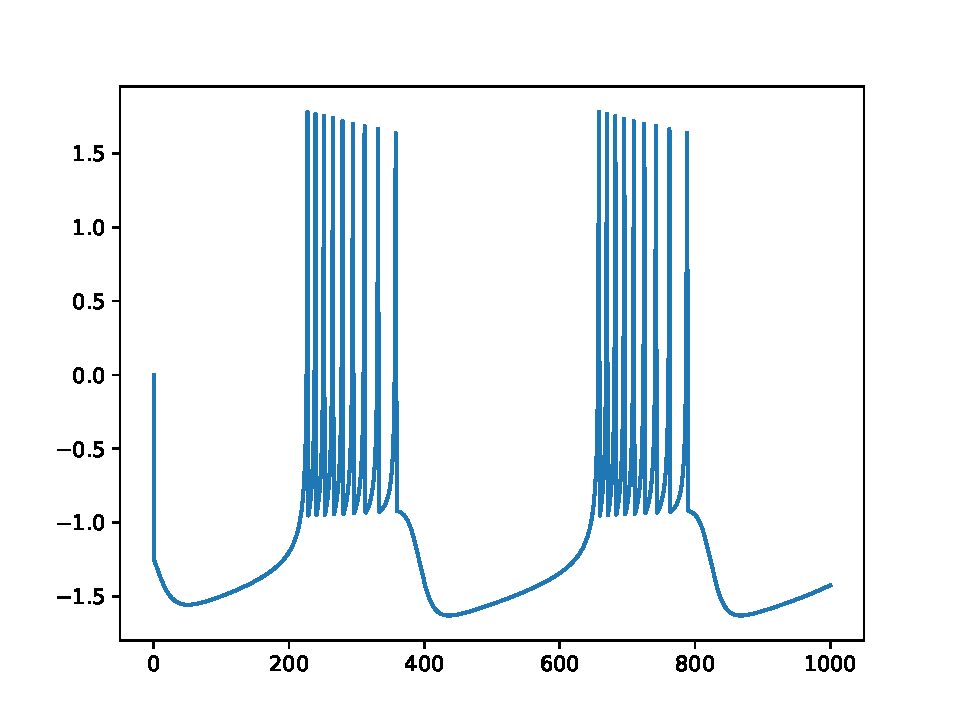
\includegraphics[trim={0cm 0.75cm 0cm 1.25cm}, clip,height=.75\textheight]{./clean_HR.pdf}
\end{center}

Ionic currents can appear to drive the neuron over bifurcations -- this is bursting!
\end{frame}

\begin{frame}[label={sec:org32f4191}]{Why do cells burst?}
\begin{itemize}
\item More reliable for transmitting over synapses
\begin{itemize}
\item Higher signal-to-noise ratio
\end{itemize}
\end{itemize}
\vfill
\begin{itemize}
\item Maintain an elevated \(Ca^{2+}\) state
\begin{itemize}
\item Promotes neurotransmitter release
\item Promotes hormone release
\end{itemize}
\end{itemize}
\vfill
\begin{itemize}
\item Occur in both the brain and elsewhere
\begin{itemize}
\item pre-Botzinger complex bursters control respiration
\item Pituitory somatotroph bursters \emph{[not neurons]} use bursts to release hormones
\end{itemize}
\end{itemize}
\end{frame}


\begin{frame}[label={sec:org515f693}]{Why do we categorise them?}
Lots of work is done to categorise bursters, but why?
\vfill
\begin{itemize}
\item Complete classification would describe all the ways a cell could be excitable
\end{itemize}
\vfill
\begin{itemize}
\item Hints at similarities and differences between cells
\begin{itemize}
\item Small parameter changes can sometimes shift cells into different burster categories
\item `Close' cell categories usually perform similar tasks
\end{itemize}
\end{itemize}
\end{frame}


\begin{frame}[label={sec:org940aad4}]{How do we categorise bursters?}
\begin{center}
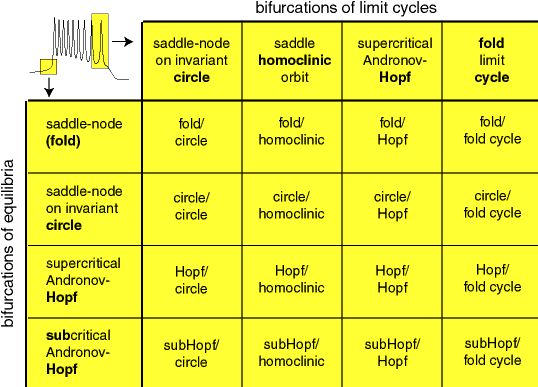
\includegraphics[height=.75\textheight]{./categories.png}
\end{center}

Under this scheme, there's 16 planar bursters
\end{frame}


\begin{frame}[label={sec:orge068efd}]{Multiple timescale dynamics}
The previous bursting data can be modelled by

\[\dot{x} = f(x,y)~,\]
\[\dot{y} = \epsilon g(x,y)~,\]
\[|\epsilon| \ll 1~.\]

\begin{itemize}
\item Assume \(\epsilon=0\)
\item Spiking is switched off by bifurcations in \(x\)
\begin{itemize}
\item \(y\) becomes a parameter to cause these bifurcations
\end{itemize}
\end{itemize}
\end{frame}


\begin{frame}[label={sec:orgf787f39}]{How do we categorise bursters?}
\begin{center}
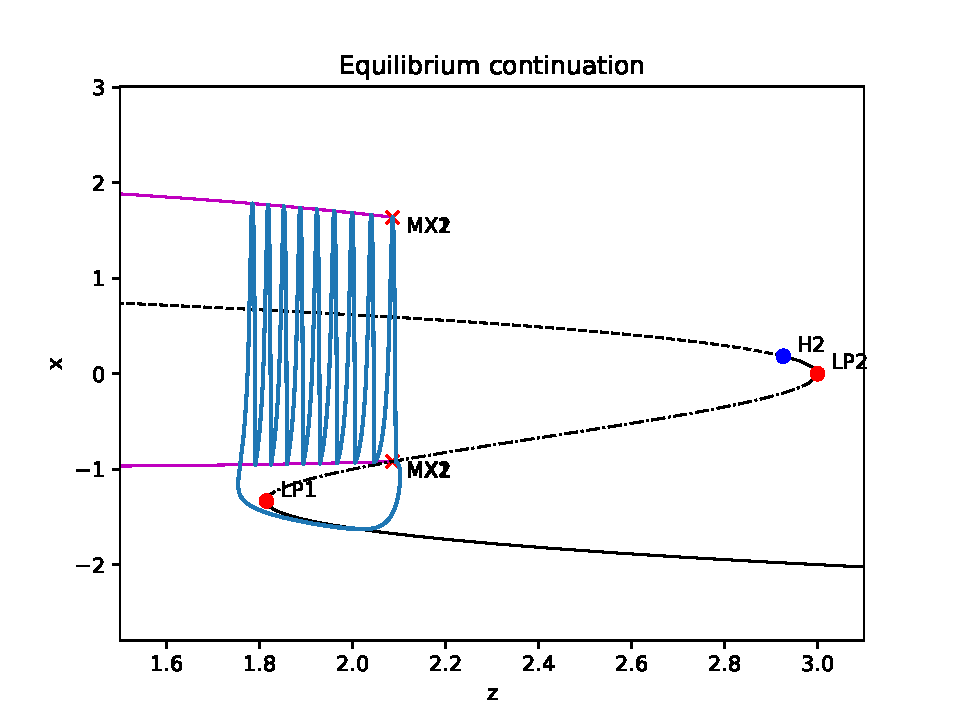
\includegraphics[trim={0cm 0.75cm 0cm 1.25cm}, clip,height=.75\textheight]{./burster_diagram.pdf}
\end{center}

This is a fold-homoclinic burster
\end{frame}



\begin{frame}[label={sec:org2ac7944}]{A better classification}
\begin{itemize}[<+->]
\item Several bifurcations can happen at the same point
\begin{itemize}
\item A singularity is a point where one or more bifurcations happen
\end{itemize}
\item If we add some small terms to a singularity \emph{(unfold it)}, we get a bifurcation space
\begin{itemize}
\item We get a model where we can vary some parameters and see some bifurcations
\end{itemize}
\item A burster will sit in the unfolding of some singularity
\begin{itemize}
\item More unfolding parameters = more complexity
\item More unfolding parameters = higher codimension
\end{itemize}
\end{itemize}
\end{frame}

\begin{frame}[label={sec:org04835f9}]{A better classification}
Classify in terms of\ldots{}
\vfill
\begin{itemize}
\item Singularity codimension
\begin{itemize}
\item Measures the complexity of the burster
\end{itemize}
\item Bifurcations to turn spikes on and off
\begin{itemize}
\item Describes the dynamics of the burster
\end{itemize}
\end{itemize}
\end{frame}

\section{Section 2}
\label{sec:org0b0361a}
\subsection{SUMMARY}
\label{sec:org7ce973a}
\begin{frame}[label={sec:org483cdbd}]{Plan de jour}
\begin{itemize}
\item 30 second intro to neurons
\item \alert{Section 2: Towards a normal form for bursting}
\item Section 3: Transitions between bursting classes
\item Section 4: Codimension-classification of pseudo-plateau bursting
\item Section 5: Conclusion
\end{itemize}
\end{frame}

\subsection{Normal forms}
\label{sec:org163ac2e}
\begin{frame}[label={sec:orge0346d5}]{Normal forms}
\begin{itemize}[<+->]
\item Biological models can be complex
\item We can often find simpler models that do the same thing
\begin{itemize}
\item \emph{`Same thing'} usually means same bifurcation structure
\end{itemize}
\item A normal form is a simple model that shows prototypical example behaviours
\item A burster normal form is a simple model that can describe the bifurcation structure of any bursting neuron \vfill
\end{itemize}

\vfill
\end{frame}

\begin{frame}[label={sec:orge456741}]{Normal form requirements}
\begin{center}
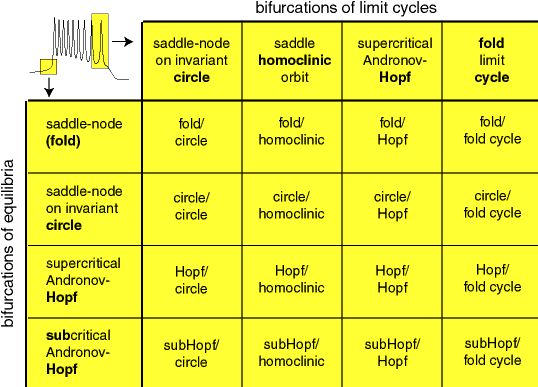
\includegraphics[height=.75\textheight]{./categories.png}
\end{center}

A burster normal form must be able to operate as all of these classes
\end{frame}

\begin{frame}[label={sec:orgbaf51c4}]{Model form}
\begin{itemize}
\item The proposed model has \(f(x,y)\) with a complex bifurcation structure\ldots{}
\end{itemize}

\[\dot{x} = f(x,y)~,\]

\begin{itemize}
\item \ldots{}and a simple \(g(x,y)\) to drive \(f\) over some bifurcations
\end{itemize}

\[y(t) = A\sin(\omega t)\]
\end{frame}

\begin{frame}[label={sec:org2a573bc}]{Appropriate models}
\begin{itemize}
\item Golubitsky found a lot of bursters near the codimension-3 degenerate Bogdanov-Takens singularity:
\end{itemize}

\[f(x,y) = \binom{\quad y\hfill}{-y + \mu x - x^3 + y(\nu + 3x + x^2)}\]

\begin{itemize}
\item Has a rich enough bifurcation structure to show most bursting types
\end{itemize}
\end{frame}

\begin{frame}[label={sec:orga6d673f}]{How about this?}
\begin{columns}
\begin{column}{0.5\columnwidth}
\begin{center}
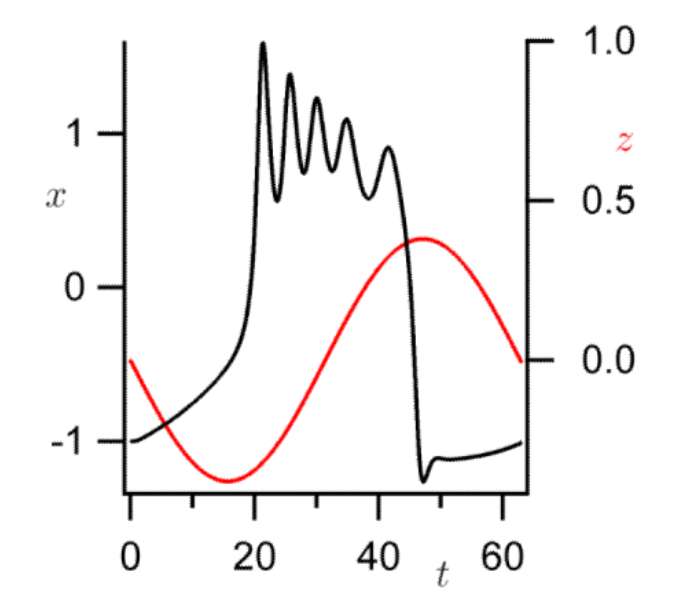
\includegraphics[width=.9\linewidth]{./PPB.png}
\end{center}
\end{column}

\begin{column}{0.5\columnwidth}
\begin{itemize}
\item Pituitory cells can also burst
\item Looks similar to previous bursters
\item No stable limit cycle!
\begin{itemize}
\item \alert{\emph{How do we categorise this?}}
\end{itemize}
\end{itemize}

\vfill

This is pseudo-plateau bursting
\end{column}
\end{columns}
\end{frame}

\begin{frame}[label={sec:org05672fa}]{The codimension of pseudo-plateau bursting}
\begin{center}
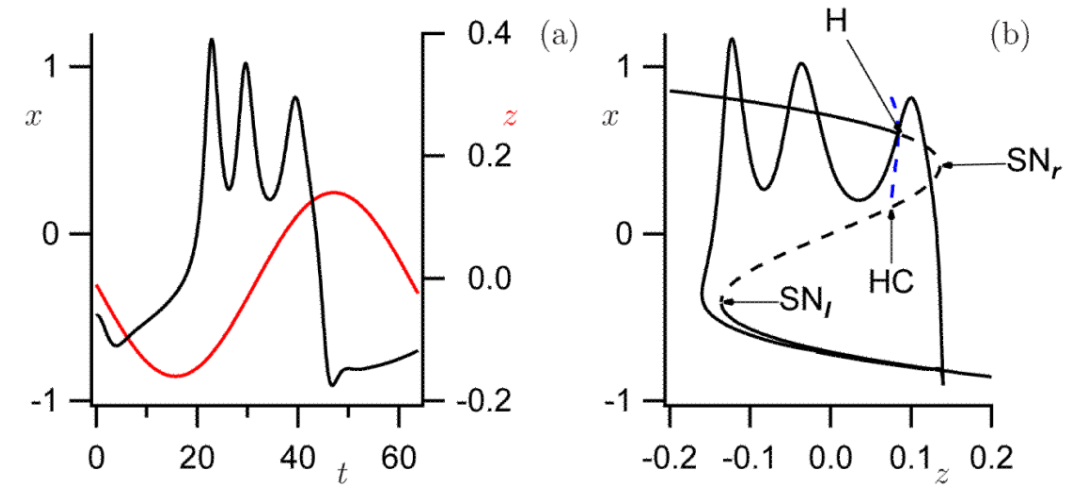
\includegraphics[width=.8\textwidth]{./psb.png}
\end{center}

\begin{itemize}
\item Pseudo-plateau bursting has a similar bifurcation structure to the others
\item It doesn't seem to appear near a degenerate Bogdanov-Takens singularity!
\end{itemize}
\end{frame}

\begin{frame}[label={sec:orgafefff9}]{Singularity choices}
\begin{itemize}
\item The original paper goal was to classify the pseudo-plateau burster
\item The burster doesn't seem to appear in codim-3 degenerate Bodganov-Takens unfolding
\begin{itemize}
\item The singularity must not be able to exhibit all known bursting types
\item It can't be a normal form!
\end{itemize}
\end{itemize}

\vfill 

Let's free up a parameter:

\[\dot{x} = \binom{\quad y \hfill}{-y + \mu_2 x - x^3 + y(\nu + bx - x^2)}\]
\end{frame}

\begin{frame}[label={sec:orgf4c4260}]{A new model}
We have

\begin{align}
\dot{x_1} &= y \nonumber \\
\dot{x_2} &= y + \mu_2 x - x^3 + y(\nu + bx - x^2) \nonumber \\
 y &= A \sin(\omega t)  \nonumber
\end{align}	

\begin{itemize}
\item This is the unfolding of a doubly-degenerate Takens-Bogdanov singularity
\item It contains more dynamical richness -- enough to show pseudo-plateau bursting
\item How do we analyse it?
\end{itemize}
\end{frame}

\begin{frame}[label={sec:orgb78f091}]{Model analysis}
We can't plot 4-dimensional bifurcation diagrams, so we need to get creative\ldots{}

\begin{itemize}[<+->]
\item The \(b\) axis consists of degenerate Bogdanov-Takens singularities
\item Small \(b\) means we're near the doubly-degenerate BT singularity
\begin{itemize}
\item We have a richer bifurcation structure in the surrounding neighbourhood than for the degenerate BT
\end{itemize}
\item Let's look for bifurcations at the edge of this small-\(b\) neighbourhood
\begin{itemize}
\item Take \(b\) small
\item Find the surface of a ball around the chosen \(b\)
\item We now have a 2d parameter space!
\end{itemize}
\end{itemize}
\end{frame}

\begin{frame}[plain,label={sec:org1802604}]{Bifurcation structure}
\begin{center}
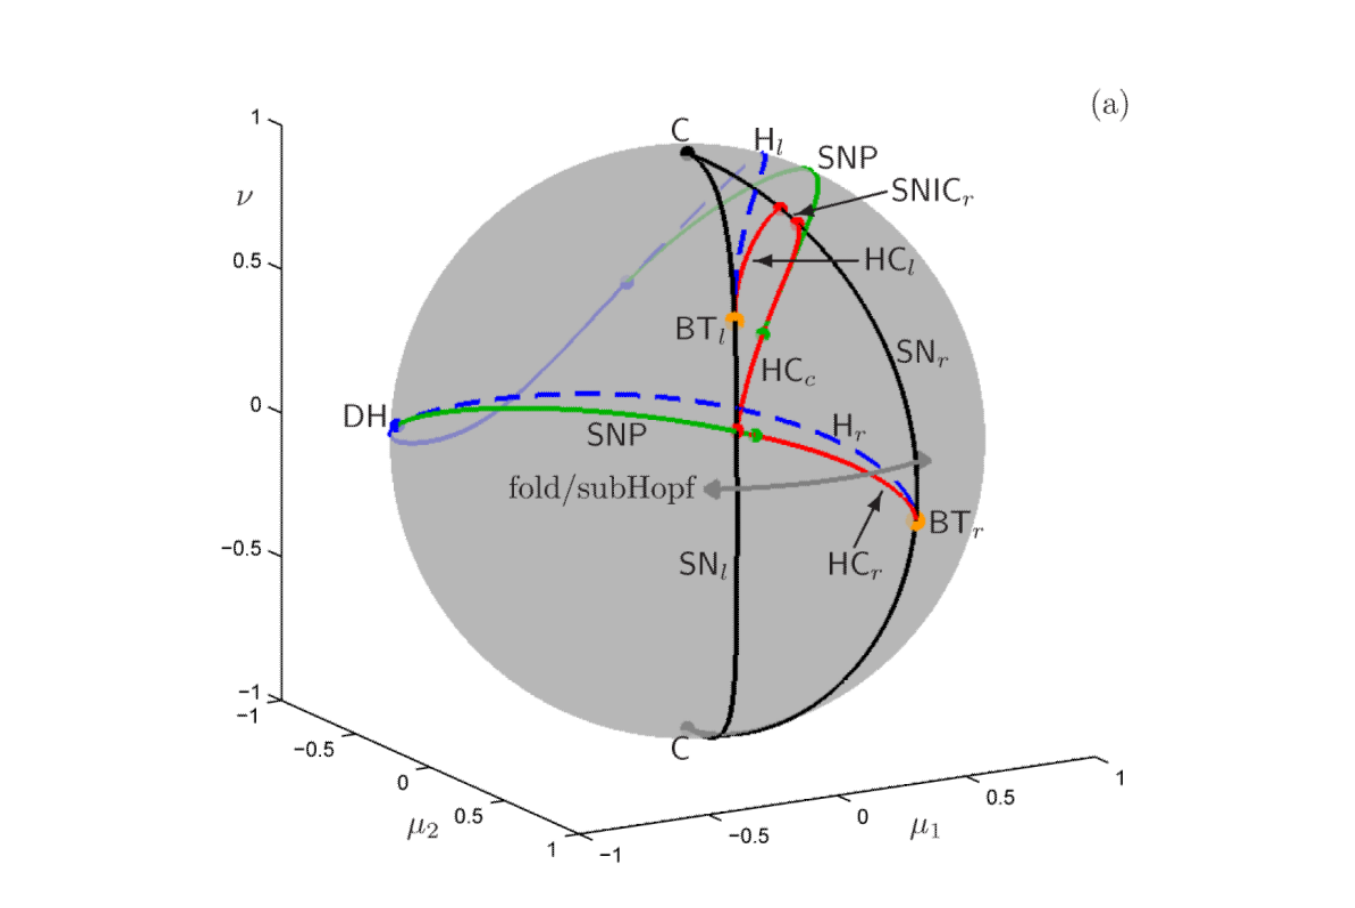
\includegraphics[width=.9\textwidth]{./bif.png}
\end{center}

\begin{itemize}
\item This parameter subspace contains the pseudo-plateau burster
\item The model is a good normal form candidate
\end{itemize}
\end{frame}

\begin{frame}[label={sec:org18ffff9}]{Section 2 summary}
\begin{itemize}[<+->]
\item A normal form is a simple model that can display a target bifurcation structure
\item The degenerate Takens-Bogdanov singularity unfolding is \emph{[probably]} not usable for a normal form
\begin{itemize}
\item The known unfoldings don't contain pseudo-plateau bursters
\item Unknown unfoldings might
\end{itemize}
\item A doubly-degenerate Bogdanov-Takens singularity \emph{does} contain pseudo-plateau bursters
\begin{itemize}
\item It is as close as we can currently get to a normal form
\end{itemize}
\end{itemize}
\end{frame}

\section{Section 3}
\label{sec:org90ed8ef}
\subsection{SUMMARY}
\label{sec:orgf235a78}
\begin{frame}[label={sec:orgd22f519}]{Plan de jour}
\begin{itemize}
\item 30 second intro to neurons
\item Section 2: Towards a normal form for bursting
\item \alert{Section 3: Transitions between bursting classes}
\item Section 4: Codimension-classification of pseudo-plateau bursting
\item Section 5: Conclusion
\end{itemize}
\end{frame}

\subsection{Section 3}
\label{sec:org0750a08}
\begin{frame}[label={sec:org49e4f05}]{We can transition between classes}
\begin{itemize}[<+->]
\item Plateau and pseudo-plateau bursting cells are similar, functionally and developmentally
\item So are their bifurcation structures: we can switch between the two classes by modifying a single parameter
\begin{itemize}
\item This parameter is analogous to Calcium current activation
\end{itemize}
\item Similar cells have similar bifurcation structures
\item Biological robustness: we can mess around with parameters and still see similar behaviour
\end{itemize}
\end{frame}

\begin{frame}[plain,label={sec:org6cc4461}]{}
\begin{center}
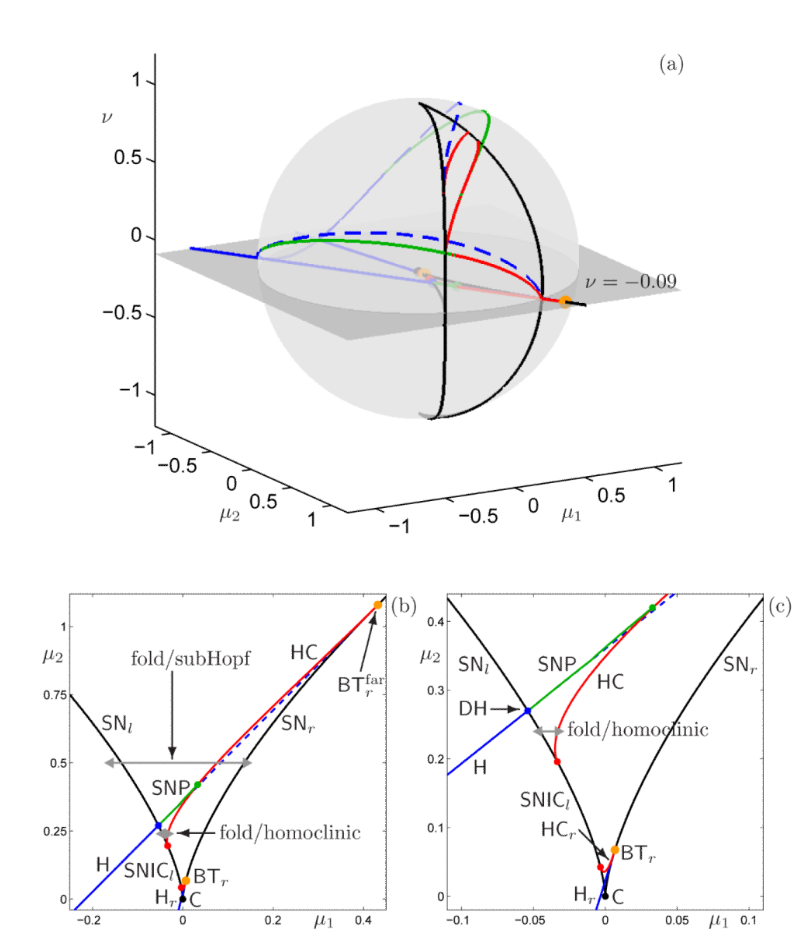
\includegraphics[height=1.4\textheight]{./3d.png}
\end{center}
\end{frame}


\section{Section 4}
\label{sec:orga660b2f}
\subsection{SUMMARY}
\label{sec:orgff164d7}
\begin{frame}[label={sec:orgc2a0426}]{Plan de jour}
\begin{itemize}
\item 30 second intro to neurons
\item Section 2: Towards a normal form for bursting
\item Section 3: Transitions between bursting classes
\item \alert{Section 4: Codimension-classification of pseudo-plateau bursting}
\item Section 5: Conclusion
\end{itemize}
\end{frame}

\subsection{Section 4}
\label{sec:org4b108c1}
\begin{frame}[label={sec:orgf7dcbca}]{Section 4}
\begin{itemize}
\item The pseudo-plateau burster appears in a codimension-4 unfolding
\begin{itemize}
\item It must be at most a codim-4 -category system
\end{itemize}
\item There's different forms the unfolding could take; this section justifies why they aren't used
\end{itemize}
\end{frame}


\section{Section 5}
\label{sec:orgae844eb}
\subsection{Section 5}
\label{sec:orgfe248d9}
\begin{frame}[label={sec:org91cd3de}]{Plan de jour}
\begin{itemize}
\item 30 second intro to neurons
\item Section 2: Towards a normal form for bursting
\item Section 3: Transitions between bursting classes
\item Section 4: Codimension-classification of pseudo-plateau bursting
\item \alert{Section 5: Conclusion}
\end{itemize}
\end{frame}

\begin{frame}[label={sec:orgd9c607f}]{Conclusions}
\begin{itemize}[<+->]
\item We can categorise bursting cells according to their codimension
\item Pseudo-plateau bursting can't be categorised as a codim-3 burster
\item The unfolding of a doubly-degenerate Bogdanov-Takens singularity can display pseudo-plateau bursting
\begin{itemize}
\item Burster must be at most codim-4
\item The singularity unfolding can act as a burster normal form
\end{itemize}
\item Cells can easily transition between bursting classes, in biologically meaningful ways
\end{itemize}
\end{frame}
\end{document}
